
\documentclass[12pt,a4paper]{article}

\usepackage{allrunes}
\usepackage{amsmath}
\usepackage[magyar]{babel}
\usepackage[T1]{fontenc}
\usepackage[utf8]{inputenc}
\usepackage{fixltx2e}
\usepackage{multirow}
\usepackage{hyperref}
\usepackage{amsfonts}
\usepackage{amsthm}
\usepackage{amssymb}
\usepackage{indentfirst}

\usepackage[a4paper]{geometry}

\geometry{a4paper,
		     tmargin = 35mm, 
		     lmargin = 25mm,
		     rmargin = 30mm,
		     bmargin = 30mm}

\theoremstyle{plain}
\usepackage{graphicx}

\usepackage{float}
\renewcommand\thesection{\Roman{section}}

\title{\textbf{Elektronspin-rezonancia}}

\author{\Large{\textsc{Olar Alex}} \vspace{10pt}\\
	\textrm{Eötvös Loránd Tudományegyetem}
	}
\date{}
%\lhead{}
\begin{document}
\addtolength{\voffset}{-1.0cm}
\addtolength{\textheight}{1.0cm}
\begin{titlepage}
    \maketitle

    \vfill

    \begin{figure}[H]
        \centering
        
\includegraphics[scale=0.6]{../elte.jpg}
    \end{figure}

    \thispagestyle{empty}
\end{titlepage}

\newpage

\linespread{1.5}

\section{A mérés célja}

\par A mérésünk a célja, hogy az elektronspinrezonancia-spekturmának mérésével
meghatározzuk a \textrm{Mn} és \textrm{Cr} ionok
giromágneses-faktorát, és a hiperfinom kölcsönhatási
együtthatókat, valamint a mintában lévő atomok számát.

\section{Elméleti leírás}

\par Az ESR mérés során Zeeman-felhadást hozunk létre
sztatikus mágneses tér segítségével. A Zeeman-nívók
között elektromágneses hullámmal átmeneteket hozunk létre.

\par Az abszorpció feltétele:

\begin{equation}
    h \nu = g \mu_{B}(B_0 + A m_I)
\end{equation}

\par Amelyben $h$ a Planck-állandó, g a g-faktor,
$\mu_B$ a Bohr-magneton.
A a finomszerkezeti állandó,
és $m_I$ a mágneses kvantumszám.

\par A mérés során $B_0$-t változtattuk és annak függvényében
figyeltük meg az abszorpciót. A mérésnél lock-in technikát
alkalmazunk, hogy ki tudjuk emelni a zajból nem kiemelkedő
jeleket. Emiatt az eljárás miatt csak a deriváltat tudjuk mérni.

\subsection{Mérési eszközök}

\begin{itemize}
    \item Elektronspinrezonancia-spektroszkóp
    \item \textrm{Mn} és \textrm{Cr} minták
\end{itemize}

\section{Kiértékelés}

\par A hiperfinom kölcsönhatás miatt az ESR 2I+1 féleképpen
történhet meg, így mindig ennyi csúcsot (derivált csúcsot)
kell keresnünk a spektrumban.

\subsection{Króm}

\par A krómnak három stabil izotópja fordul elő:
$\textrm{Cr}^{52}$, $\textrm{Cr}^{53}$, illetve
$\textrm{Cr}^{54}$. Ezek közül $\textrm{Cr}^{52}$ a
leggyakoribb.

\par Két spektrumot rögzítettünk, egy
teljest és egyet ami a legnagyobb csúcsra
helyezkedik. A teljes ben a nagy csúcs mellett jobbra
kivehető kis kiszögellést tekintettem kisebb csúcsnak
mivel ezeket az idő rövidsége miatt nem sikerült
érdemben lemérni.

\begin{figure}[H]
    \centering
    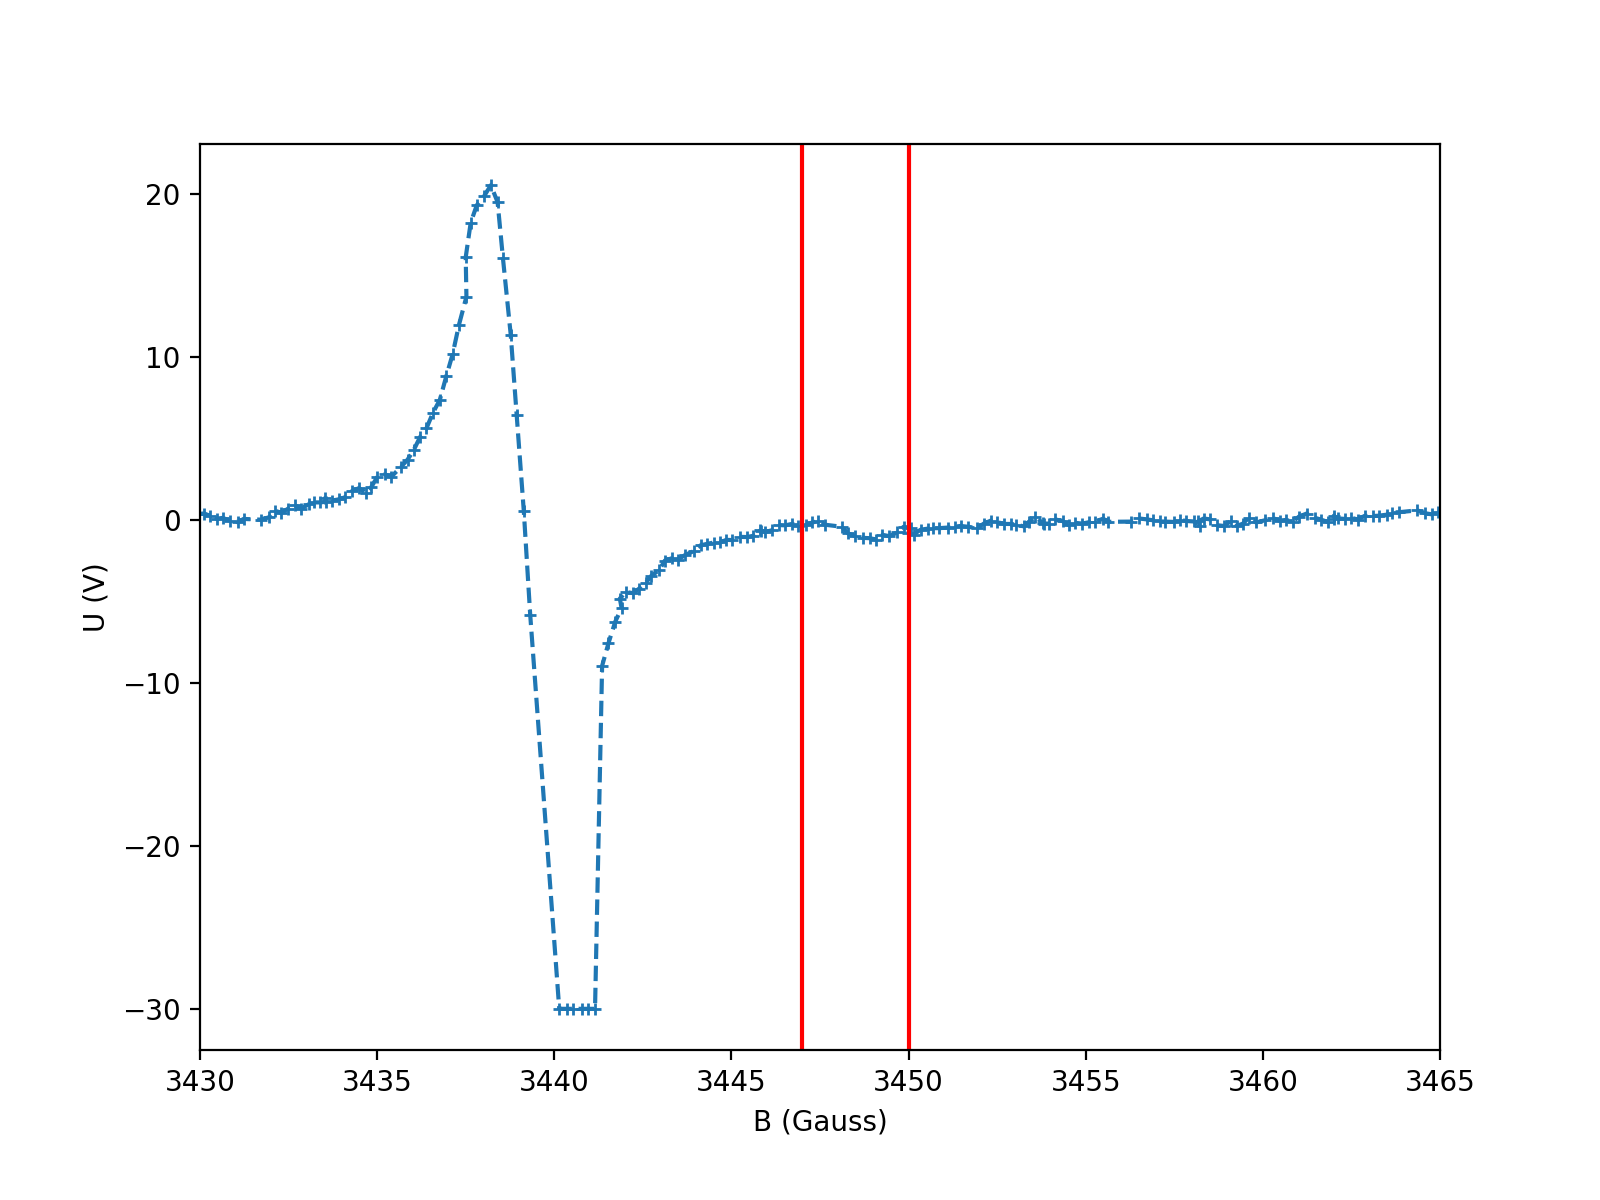
\includegraphics[width=.6\linewidth]{./alex_cromium.png}
    \caption{Cr 5. csúcs}
\end{figure}

\par Az ábrán jelölve van az illesztett
kiszögellés.

\par Az Lorentz-görbe a következő alakú:
\[  f(x) = \frac{a}{(1+s(x-x_0)^2)}\]

\par Ennek deriváltja amit illesztettünk:
\[ \frac{df}{dx} = \frac{-2as(x-x_0)}{(1+s(x-x_0)^2)^2} (+ c)\]

\par A mérés során felvettük a teljes spektrumot.

\par A \textrm{Cr}-mintában lévő atomok száma:

\begin{equation*}
    N_{\textrm{Cr}} = 8,3 \cdot 10^{13}
\end{equation*}

\par A \textrm{Cr} g-faktora is ismert:

\begin{equation}
    g_{\textrm{Cr}}=1.98 \pm 0.0001
\end{equation}

\par A minta a $\textrm{Cr}^{52}$ mellett tartalmaz
megközelítőleg 1/5 arányban $\textrm{Cr}^{53}$-t is.
Emiatt a középső nagy csúcs mellett megjelenik négy kisebb
csúcs is a spektrumban.

\par A rendkívül kevés idő miatt csak a teljes spektrumot
sikerült jól lemérni és a legnagyobb csúcsot lehetett csak
pontosan illeszteni. Egy kisebb csúcsot találomra
választva pedig azt is illesztetük.

\begin{figure}[H]
    \centering
    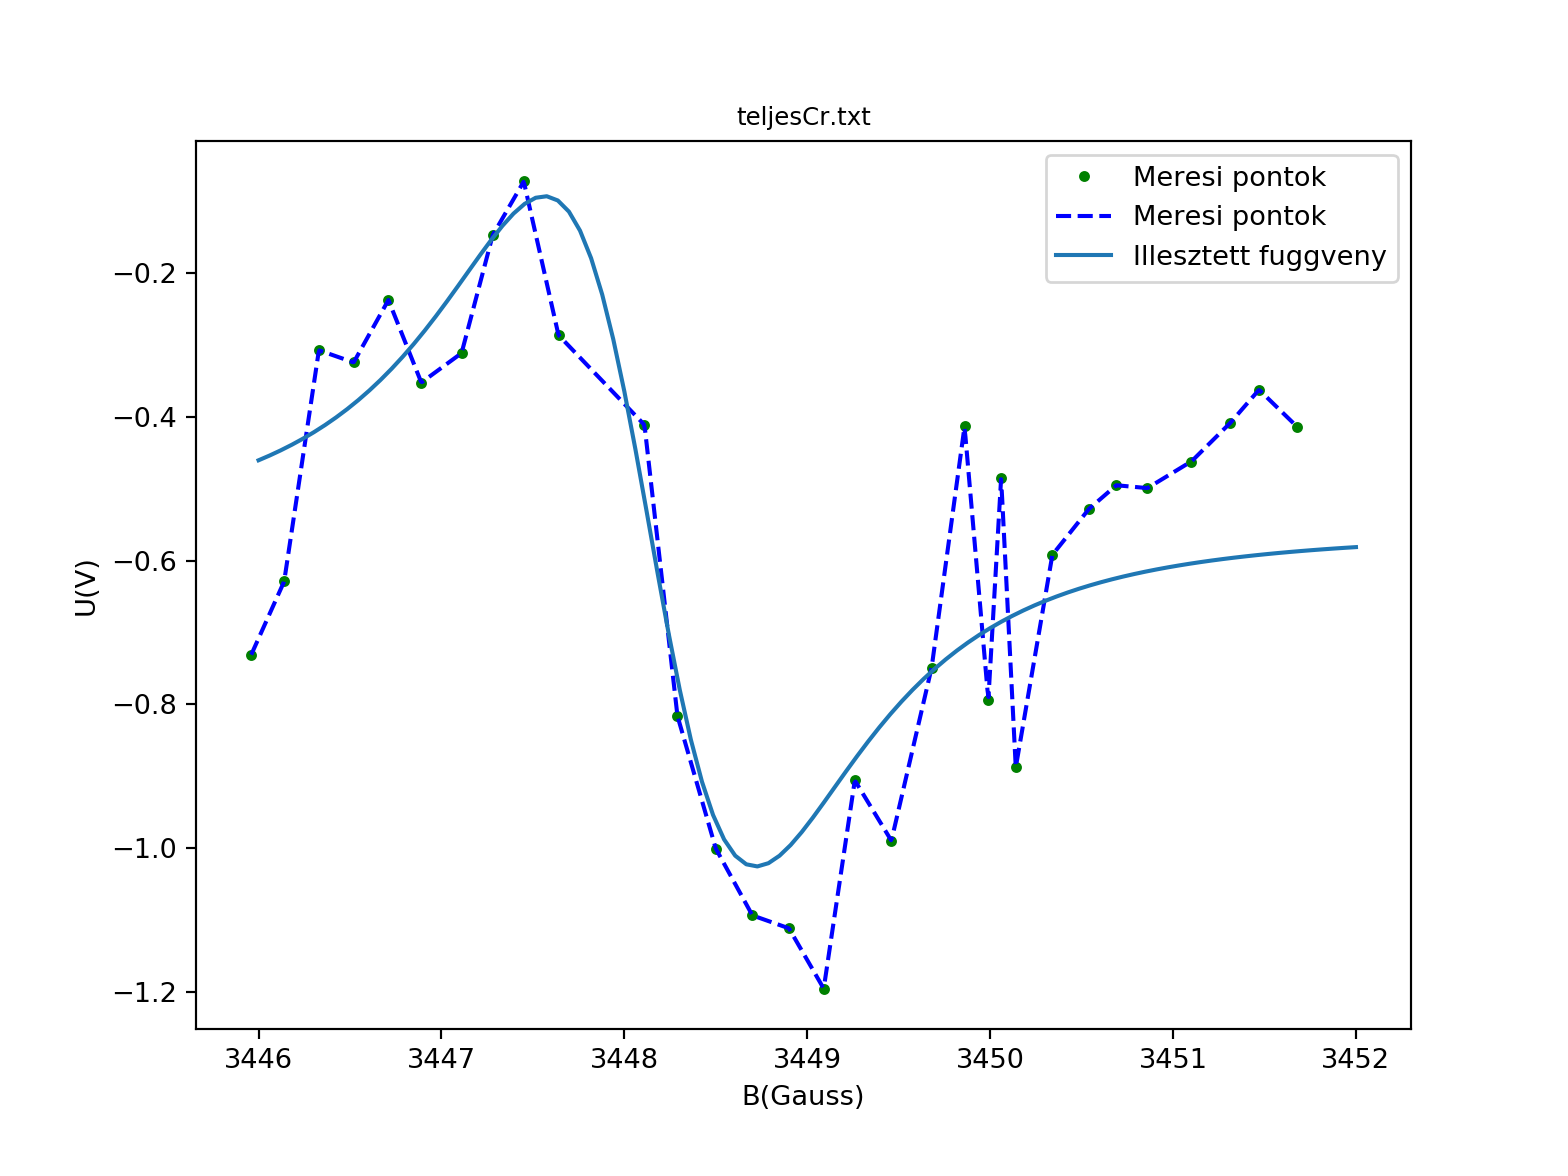
\includegraphics[width=.65\linewidth]{./images/alex_meres_cr_small.png}
    \caption{Cr - kis csúcs}
\end{figure}

\begin{figure}[H]
    \centering
    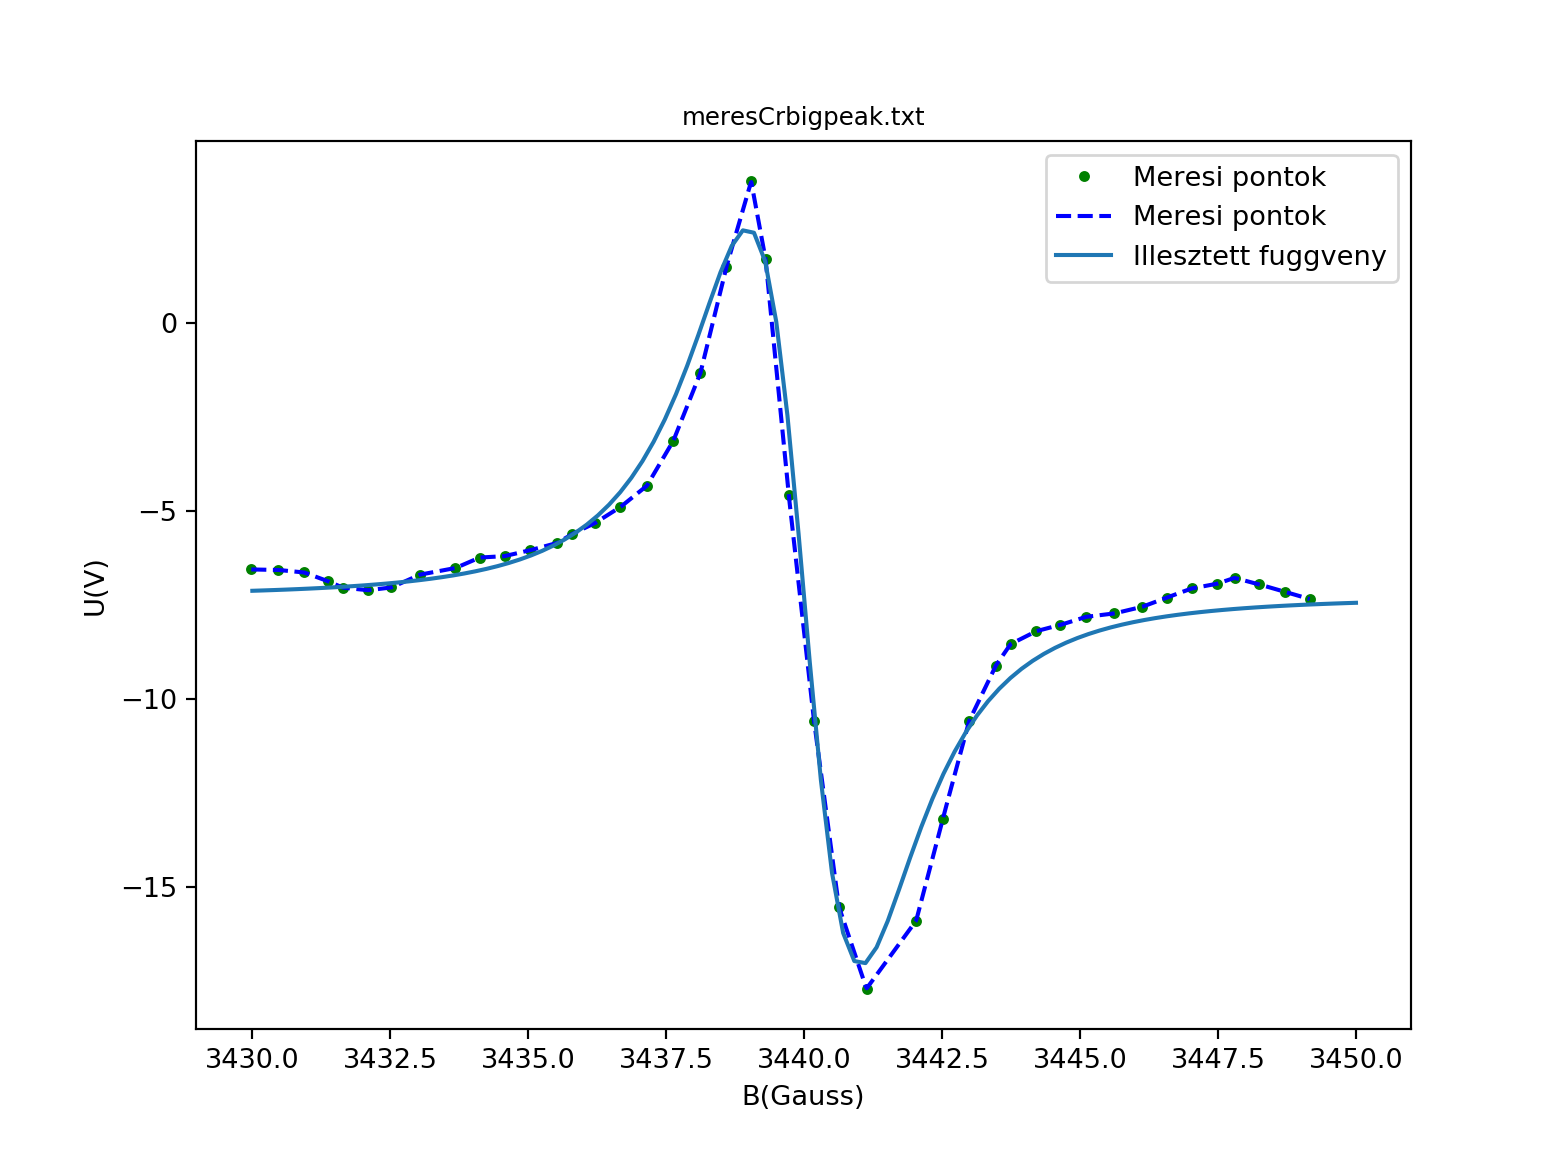
\includegraphics[width=.65\linewidth]{./images/alex_meres_cr_big.png}
    \caption{Cr legnagyobb csúcs}
\end{figure}

\par Az illesztett paraméterek
a következők:

\begin{table}[H]
    \begin{center}
        \begin{tabular}{|c|c|c|c|c|c|c|c|}
            \hline
            $a$                  & $s$                 & $x_0$                  & $c$                  \\ \hline
            $0.719 \pm 0.00016$  & $0.998 \pm 0.00129$ & $3448.141 \pm 0.00007$ & $-0.559 \pm 0.00002$ \\ \hline
            $26.829 \pm 0.02674$ & $0.316 \pm 0.00001$ & $3439.998 \pm 0.00003$ & $-7.278 \pm 0.00046$ \\ \hline
        \end{tabular}
        \label{tab:3}
    \end{center}
\end{table}

\par A \textrm{Cr} kis csúcsa $\approx$ 1/66-ed
területű a nagy csúcshoz képest. Az illesztésből:

\begin{equation}
    T_{\textrm{Cr}}^{nagy}= 149.94 \pm 0.005
\end{equation}

\begin{equation}
    T_{\textrm{Cr}}^{kicsi}= 2.26 \pm 0.005
\end{equation}

\par A fentebbi adatok a Lorentz-görbe alatti területek,
melyeket a Wolfram Alpha programmal integráltam, 
beillesztve a megfelelő paramétereket.

\par Ebből a foton frekvenciája:

\begin{equation}
    \nu = \dfrac{g_{\textrm{Cr}}\cdot\mu_{B}\cdot m}{h} = 9.0373 GHz
\end{equation}

\subsection{Mangán}

\par A mérés ezen részében a $^{55}\textrm{Mn}^{+2}$
mintát vizsgáljuk, a teljes spektrum itt látható:

\begin{figure}[H]
    \centering
    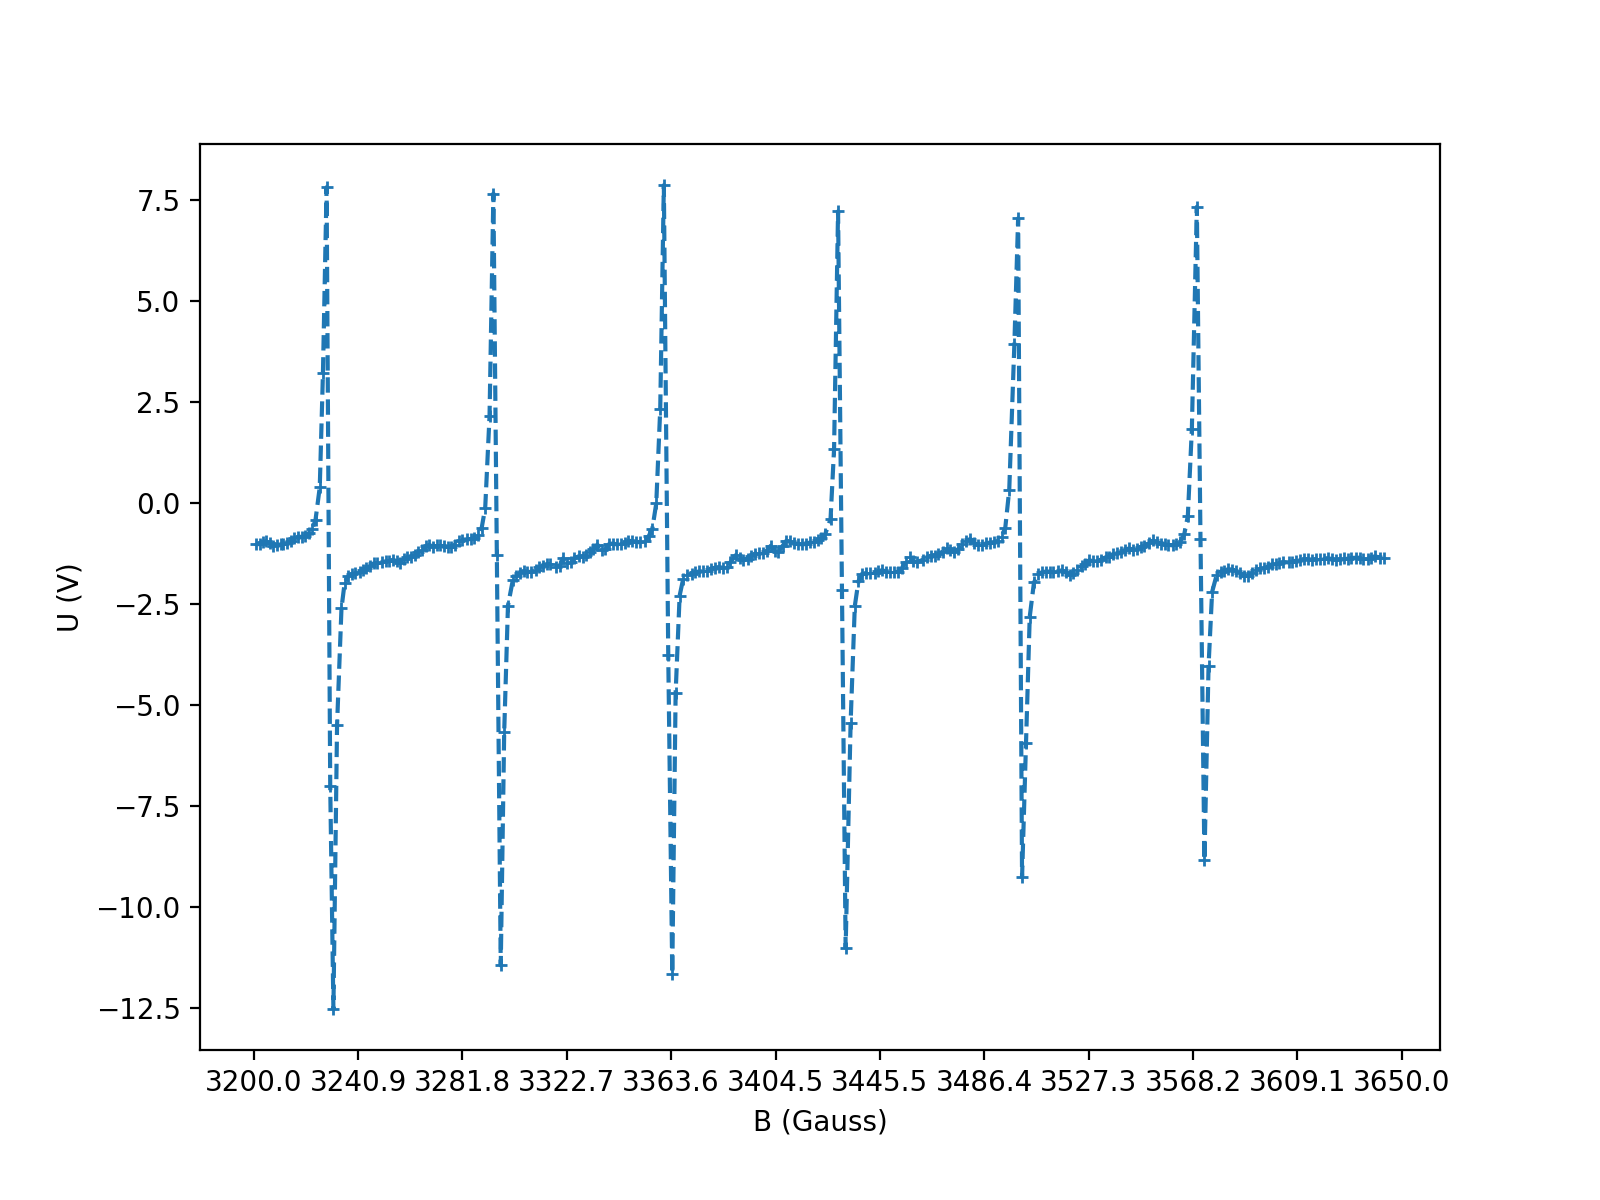
\includegraphics[width=.9\linewidth]{./alex_manganese.png}
    \caption{Mangán}
\end{figure}

\par Ezen spektrum minden egyes dupla csúcsára Lorentz-görbe
deriváltat illesztettünk. Eredményeink a következők:

\begin{table}
    \begin{center}
        \begin{tabular}{|c|c|c|c|c|} \hline
            $m$    & $a$                  & $s$                 & $x_0$                  & $c$                  \\ \hline
            $-2.5$ & $28.788 \pm 0.04772$ & $0.218 \pm 0.00001$ & $3229.567 \pm 0.00007$ & $-1.517 \pm 0.00040$ \\ \hline
            $-1.5$ & $26.738 \pm 0.03633$ & $0.192 \pm 0.00001$ & $3295.331 \pm 0.00007$ & $-1.380 \pm 0.00021$ \\ \hline
            $-0.5$ & $27.546 \pm 0.05404$ & $0.178 \pm 0.00001$ & $3362.214 \pm 0.00010$ & $-1.373 \pm 0.00040$ \\ \hline
            $0.5$  & $27.429 \pm 0.04850$ & $0.172 \pm 0.00001$ & $3430.565 \pm 0.00009$ & $-1.519 \pm 0.00034$ \\ \hline
            $1.5$  & $22.995 \pm 0.00679$ & $0.261 \pm 0.00000$ & $3500.397 \pm 0.00001$ & $-1.205 \pm 0.00007$ \\ \hline
            $2.5$  & $24.141 \pm 0.02856$ & $0.174 \pm 0.00001$ & $3571.142 \pm 0.00007$ & $-1.151 \pm 0.00024$ \\ \hline
        \end{tabular}
    \end{center}
\end{table}

\par Az illesztések numerikus stabillá tételéhez a
következő módszereket alkalmaztuk. Mivel a adatsor
az idő rendkívüli rövidsége miatt nem volt megfelelően
vételezve, ezért az illesztés során interpoláltuk a
meglévő adatokból a köztes pontokat így lehetővé téve,
hogy illeszhető görbéket kapjunk. Nagyban hozzájárul az
illesztés pontosságához, hogy $mV$-ról áttértünk $V$-ra,
hiszen ez numerikusan jóval stabilabbá tette a
számolást.

\par Ezekből a számolt területek:
\begin{table}[H]
    \begin{center}
        \begin{tabular}{|c|c|}
            \hline
            $\textrm{mérés}$ & $T$                            \\ \hline
            $1$ & $193.554 \pm 45.240$ \\ \hline
            $2$ & $191.616 \pm 41.655$ \\ \hline
            $3$ & $205.070 \pm 56.465$ \\ \hline
            $4$ & $207.913 \pm 55.221$ \\ \hline
            $5$ & $141.337 \pm 11.387$ \\ \hline
            $6$ & $181.596 \pm 36.725$ \\ \hline
        \end{tabular}
        \caption{Lorentz-görbe alatti területek}
        \label{tab:2}
    \end{center}
\end{table}

Ha a mágneses kvantumszám függvényében ábrázoljuk a \textrm{Mn} illesztéséből származó csúcsok helyeit. Akkor egy lineáris függvényt kaptunk ahol:

\begin{equation}
    B_0 = - \dfrac{A}{g_M \mu_B} \cdot m_I + \dfrac{h \nu}{g_M \mu_B}
\end{equation}

Tehát a függvény meredekségéből és tengelymetszetéből meghatározhatók akívánt értékek.
Az illesztéshez a gnuplot nevű programot használtuk.

Az illesztési paraméterek a következők:
\begin{equation}
    a  = -68.326 \pm 0.552 \quad \quad b = 3398.2026 \pm 0.8317
\end{equation}

Ez alapján a kívánt értékek:

\begin{equation}
    g_{M_n}= -\dfrac{h \nu}{\mu_{B} b}= 2.1354 \pm 0.0005
\end{equation}

\begin{equation}
    A=-ag_{M_n} \cdot \mu_{B} = (1.327 \pm 0.01) \cdot 10^{-25} ~J
\end{equation}

\subsubsection{\textrm{Mn}-atomok számának meghatározása}

A 6 csúcs alatti terület összege: $T_{M_n}$

Mivel a \textrm{Cr} spektrumot 1mV-os méréshatárral mértük. Ezért a területek arányát meg kell szorozni 5-tel.

\begin{center}
    \begin{equation}
        N_{M_n}= N_{\textrm{Cr}} \cdot 5 \cdot\dfrac{T_{M_n}}{T_{\textrm{Cr}}}=(5.8609 \pm 0.012) \cdot 10^{15} J
    \end{equation}
\end{center}

\section{Bónusz feladatok}

\textbf{1.} \textit{A legtöbb ESR-spektrométer $10$ GHz frekvencián és kb. $0.3$ T mágneses térnél mûködik. Milyen elõnyei illetve hátrányai lennének
ha feljebb, illetve lejebb mennénk.}

\vspace{5mm}

\par Célszerû a két paramétert, bár anyagonként szorosan csatolt mégis külön tárgyalni. Frekvencia esetében amennyiben lefelé mennénk egyre
nagyobb fizikai méreteket öltene a rendszer, mivel a \emph{waveguide}-ok mérete a frekvencia reciprokával növekednek. Némi elõnyt jelentene,
hogy lassabb válaszidejû elemeket is lehetne alkalmazni, illetve az alacsonyabb frekvenciákon mûködõ oszcillátorok pontosabbak. Nagyobb
frekvencia esetén a legnagyobb nyereség a fizika méreteken lenne, ám cserébe bonyolultabb elektronikát és más detektorokat kellene használnunk.

\par Mágneses tér esetén amennyiben kisebb tereket állítanánk elõ sokkal kevesebb anyagból megoldható lenne az elektromágnes, ezzel mind kisebb,
mind jóval könnyebb és költséghatékonyabb lenne a rendszer. Hátránya az volna, hogy az amúgy is kis effektusnak számító rezonancia intenzitása
leesne. Nagy mágneses térnél megkerülhetetlen a szupravezetõ mágnesek használata, melyek viszont a használatukhoz hélium rendszert is igényelnek.
Az egész konstrukció így meglehetõsen drága és rugalmatlan. Nyilván nagy mágneses tér esetén, gyengébb átmenetek is gond nélkül vizsgálhatóak.

\par Amennyiben egy adott anyagra nézzük a frekvencia, mágneses tér párt, úgy leginkább mindkettõ növelésébõl profitálnánk, mivel ekkor
nõne a jel intenzitása. Megjegyezzük továbbá, hogy a legtöbb disszipáció a frekvenciával arányos, így magasabb frekvenciájú spektrométer
mûködtetéséhez több energiát is kellene befektetni.

\vspace{5mm}

\textbf{2.} \textit{Miért $100$ kHz a Lock-In modulációjának sebessége?}

\vspace{5mm}

\par A Lock-In modulációs sebességét elsõsorban az üreg sávszélessége, azaz fizikai méretei határozzák meg. Amennyiben túl gyorsan
modulálnánk az üreget hagyományos értelemben nem kapnánk választ, az üregben lévõ térnek nincs ideje felépülnie. Ilyen esetekben
elterjedt az optikából jól ismert PDH (Pound--Drever--Hall) módszer.

\par Egyéb korlátozó tényezõ lehet a diódák karakterisztikája, illetve, hogy az alacsonyabb frekvenciákon üzemelõ Lock-In-ok maximális
modulációs sebessége $100$ kHz, a magas frekvenciás Lock-In erõsítõk pedig jelentõsen drágábbak.

\vspace{5mm}

\textbf{3.} \textit{Miért Lorentz görbénk van és nem Gauss?}

\vspace{5mm}

\par Rezonancia csúcsoknál mindig Lorentz görbét alkalmazunk 
fizikában, hiszen ez jellemzi jól egy csúcs helyét, szélességét
és nagyságát. Gauss görbét valamiféle feltételezett eloszlásra szoktunk 
illeszteni, amikor az adatoknak nem feltétlenül van egy kiugró pontjuk.

\vspace{5mm}

\textbf{4.} \textit{H atom ESR spektruma?}

\vspace{5mm}

\par A hidrogénatom alapállapoti konfigurációja 1s$^1$, azaz feles spinû. Mivel a magja egyetlen protonból áll, így magspinje is feles. 
A kiválasztási szabályokat kielégítve ilyen módon kétféle átmenet valósulhat meg, azaz két csúcsot kapunk a spektrumban.

\par A spin-spin csatolási állandó arányos a csúcsok távolságával. Míg H esetén a két csúcs távolsága $400-500$ G, addig Mn esetén $50-60$ G-t
tapasztaltunk. Ennek oka, hogy az egyetlen elektron sokkal erõsebben tud csatolni a maggal, mint egy sokelektronos rendszer külsõ elektronjai.

\section{Diszkusszió}

\par Ez a labor volt a BSc-s laborokkal együtt a 7.
laborom és ebben a félévben az ESR volt  legszörnyűbb mérés.
Alapvetően nem mértünk semmit, amit mértünk azt is rosszul, kutyafuttában,
mert elbeszéltük az időt, ami nem is lenne baj feltétlenül, ha ezalatt futtathattuk volna a mérést.
Összesen két spektrumra volt szükségünk, ezek mindegyike megfelelő sűrűen vételezhető lett volna
2-2 óra alatt a teljes tartományban, mi ennek ellenére a labor utolsó 40 percében próbáltuk kitalálni, hogy 
hogyan lehet gyorsan mérni. Nem csak, hogy ez volt az utolsó mérésünk, de tovább tartott fél órával, mivel 
a hibás adatok mellett azok továbbítása is egy ősrégi, használhatatlan gépen történt. A labort fél órával az
óra hivatalos vége után hagyták el társaim (12:15), mivel 15 percig tartott a böngészőn behozni egy webes email
klienst. 

\par A sorozatos rossz élmények után egyből levelet intéztem a labor vezetői felé, amire készségesen reagáltak.
Én teljes mértékben megértem, hogy az egyetemnek nincs anyagi forrása a laborok korszorűsítésére, de ha ez így van
akkor van egy kézen fekvő megoldás. Miután elvégeztünk egy BSc-t és szakasodunk, semmi szükség nincs arra, hogy
görbéket illesztgessek, hiszen ez már készség szinten megy. Eljutottam odáig, hogy 
a hibás adatokat interpolálva még így is tudtam görbét illeszteni. Hibaszámítást már 3 éve tudjuk korrektül
csinálni, de nem fogjuk, mert egyszerűen túl sok időt vesz igénybe. Javaslom a laborok megszűntetését. Ezzel ha 
szükséges legalább fleszabadulnak a műszerek, nem teszik tönkre a hallgatók és használhatja az akinek szüksége van rá,
bár felteszem ez elenyésző számú kutató még a fizikusok között is, hiszen ma már mindenki a programoz, 
részecskegyorsítók adatait elemzi vagy elméleteket gyárt papíron.

\par A bónusz kérdések megoldásai lassan 10 éve elérhetőek az interneten.
Nagyjából 10 perc volt megtalálni és összeszerkeszteni őket. Én nagyon sajnálom, hogy ez a helyzet,
de úgy érzem, hogy ez is mutatja, hogy nem hasznosan töltjük el az egyetem által ránk szabott időnket.

\clearpage


\end{document}
